%%
%% This is file `sample-manuscript.tex',
%% generated with the docstrip utility.
%%
%% The original source files were:
%%
%% samples.dtx  (with options: `all,proceedings,bibtex,manuscript')
%% 
%% IMPORTANT NOTICE:
%% 
%% For the copyright see the source file.
%% 
%% Any modified versions of this file must be renamed
%% with new filenames distinct from sample-manuscript.tex.
%% 
%% For distribution of the original source see the terms
%% for copying and modification in the file samples.dtx.
%% 
%% This generated file may be distributed as long as the
%% original source files, as listed above, are part of the
%% same distribution. (The sources need not necessarily be
%% in the same archive or directory.)
%%
%%
%% Commands for TeXCount
%TC:macro \cite [option:text,text]
%TC:macro \citep [option:text,text]
%TC:macro \citet [option:text,text]
%TC:envir table 0 1
%TC:envir table* 0 1
%TC:envir tabular [ignore] word
%TC:envir displaymath 0 word
%TC:envir math 0 word
%TC:envir comment 0 0
%%
%% The first command in your LaTeX source must be the \documentclass
%% command.
%%
%% For submission and review of your manuscript please change the
%% command to \documentclass[manuscript, screen, review]{acmart}.
%%
%% When submitting camera ready or to TAPS, please change the command
%% to \documentclass[sigconf]{acmart} or whichever template is required
%% for your publication.
%%
%%
\documentclass[manuscript,screen,review]{acmart}
\usepackage{indentfirst} % 必须添加
%%
%% \BibTeX command to typeset BibTeX logo in the docs
\AtBeginDocument{%
  \providecommand\BibTeX{{%
    Bib\TeX}}}

%% Rights management information.  This information is sent to you
%% when you complete the rights form.  These commands have SAMPLE
%% values in them; it is your responsibility as an author to replace
%% the commands and values with those provided to you when you
%% complete the rights form.
\setcopyright{acmlicensed}
\copyrightyear{2018}
\acmYear{2018}
\acmDOI{XXXXXXX.XXXXXXX}
%% These commands are for a PROCEEDINGS abstract or paper.
\acmConference[Conference acronym 'XX]{Make sure to enter the correct
  conference title from your rights confirmation email}{June 03--05,
  2018}{Woodstock, NY}
%%
%%  Uncomment \acmBooktitle if the title of the proceedings is different
%%  from ``Proceedings of ...''!
%%
%%\acmBooktitle{Woodstock '18: ACM Symposium on Neural Gaze Detection,
%%  June 03--05, 2018, Woodstock, NY}
\acmISBN{978-1-4503-XXXX-X/2018/06}


%%
%% Submission ID.
%% Use this when submitting an article to a sponsored event. You'll
%% receive a unique submission ID from the organizers
%% of the event, and this ID should be used as the parameter to this command.
%%\acmSubmissionID{123-A56-BU3}

%%
%% For managing citations, it is recommended to use bibliography
%% files in BibTeX format.
%%
%% You can then either use BibTeX with the ACM-Reference-Format style,
%% or BibLaTeX with the acmnumeric or acmauthoryear sytles, that include
%% support for advanced citation of software artefact from the
%% biblatex-software package, also separately available on CTAN.
%%
%% Look at the sample-*-biblatex.tex files for templates showcasing
%% the biblatex styles.
%%

%%
%% The majority of ACM publications use numbered citations and
%% references.  The command \citestyle{authoryear} switches to the
%% "author year" style.
%%
%% If you are preparing content for an event
%% sponsored by ACM SIGGRAPH, you must use the "author year" style of
%% citations and references.
%% Uncommenting
%% the next command will enable that style.
%%\citestyle{acmauthoryear}


%%
%% end of the preamble, start of the body of the document source.
\begin{document}

%%
%% The "title" command has an optional parameter,
%% allowing the author to define a "short title" to be used in page headers.
\title{The Name of the Title Is Hope}

%%
%% The "author" command and its associated commands are used to define
%% the authors and their affiliations.
%% Of note is the shared affiliation of the first two authors, and the
%% "authornote" and "authornotemark" commands
%% used to denote shared contribution to the research.
\author{Zheng Li}
\authornote{Both authors contributed equally to this research.}
\affiliation{
  \institution{Southeast University}
  \city{Nanjing}
  \country{China}
}
\email{LiZheng040910@163.com}

%%
%% By default, the full list of authors will be used in the page
%% headers. Often, this list is too long, and will overlap
%% other information printed in the page headers. This command allows
%% the author to define a more concise list
%% of authors' names for this purpose.
\renewcommand{\shortauthors}{Trovato et al.}

%%
%% The abstract is a short summary of the work to be presented in the
%% article.
\begin{abstract}

\end{abstract}

%%
%% The code below is generated by the tool at http://dl.acm.org/ccs.cfm.
%% Please copy and paste the code instead of the example below.
%%
% \begin{CCSXML}
% <ccs2012>
%  <concept>
%   <concept_id>00000000.0000000.0000000</concept_id>
%   <concept_desc>Do Not Use This Code, Generate the Correct Terms for Your Paper</concept_desc>
%   <concept_significance>500</concept_significance>
%  </concept>
%  <concept>
%   <concept_id>00000000.00000000.00000000</concept_id>
%   <concept_desc>Do Not Use This Code, Generate the Correct Terms for Your Paper</concept_desc>
%   <concept_significance>300</concept_significance>
%  </concept>
%  <concept>
%   <concept_id>00000000.00000000.00000000</concept_id>
%   <concept_desc>Do Not Use This Code, Generate the Correct Terms for Your Paper</concept_desc>
%   <concept_significance>100</concept_significance>
%  </concept>
%  <concept>
%   <concept_id>00000000.00000000.00000000</concept_id>
%   <concept_desc>Do Not Use This Code, Generate the Correct Terms for Your Paper</concept_desc>
%   <concept_significance>100</concept_significance>
%  </concept>
% </ccs2012>
% \end{CCSXML}

% \ccsdesc[500]{Do Not Use This Code~Generate the Correct Terms for Your Paper}
% \ccsdesc[300]{Do Not Use This Code~Generate the Correct Terms for Your Paper}
% \ccsdesc{Do Not Use This Code~Generate the Correct Terms for Your Paper}
% \ccsdesc[100]{Do Not Use This Code~Generate the Correct Terms for Your Paper}

%%
%% Keywords. The author(s) should pick words that accurately describe
%% the work being presented. Separate the keywords with commas.
\keywords{Do, Not, Us, This, Code, Put, the, Correct, Terms, for,
  Your, Paper}
%%
%% This command processes the author and affiliation and title
%% information and builds the first part of the formatted document.
\maketitle

\section{Introduction}

\subsection{Motivation of AI in Software Testing}

\subsection{AI as a Tool for Testing Traditional Systems}

\section{AI-Driven Test Data Generation}

\subsection{Data Augmentations for Edge Cases}

\subsection{Generative AI for Synthetic Data}

\subsection{Adversarial Sample Generation}

\section{AI-Powered Test Case Optimization}
\label{sec:3}

This chapter will detail how to leverage artificial intelligence techniques in software testing, specifically focusing on optimization methods based on Boundary Coverage Distance (BCD) and techniques using Reinforcement Learning (RL), to achieve intelligent test case generation and boundary exploration. First, in the introduction, we present the background and significance of this chapter. Then, this section is divided into two core subsections, which respectively introduce BCD-optimized boundary value analysis and the application of reinforcement learning in test exploration. Finally, we summarize and prospect the content of this chapter.

As software systems become increasingly complex and the requirements for reliability and safety continue to rise, traditional test case design methods that rely on manual experience can no longer meet practical needs. On one hand, traditional equivalence class partitioning and Boundary Value Analysis (BVA) methods, when facing high-dimensional and multi-branch complex software, require manual extraction of a large number of boundary conditions, which is extremely challenging and inefficient. On the other hand, Random Testing (RT) and Adaptive Random Testing (ART), although able to improve test coverage to some extent, still lack exploration capability for boundary defects. Therefore, how to maximize the coverage of potential boundary defect areas in software while ensuring test efficiency has become a pressing challenge in the field of software engineering.

AI-driven test case optimization emerges in this context. On one hand, by quantifying the boundary coverage with a metric like Boundary Coverage Distance (BCD), test case design can be transformed into an optimization problem, allowing intelligent algorithms to automatically search for optimal test points in the input domain. On the other hand, intelligent techniques such as reinforcement learning can dynamically construct environments and testing strategies, interacting with the system under test to efficiently approach failure boundaries and uncover defects in extreme scenarios. Combining both approaches not only reduces the manual workload of testers but also achieves more comprehensive and precise boundary testing in high-dimensional complex scenarios.

This chapter aims to clarify the principles and application effects of two main AI-driven methods for test case generation and boundary exploration. First, we will delve into BCD-based boundary value analysis, including the mathematical definition of BCD, its computation method, and the implementation of test case auto-generation using MCMC (Markov Chain Monte Carlo) optimization strategies. Then, considering dynamic scenarios such as autonomous driving, we will discuss the advantages of reinforcement learning in test exploration, emphasizing the necessity of dynamic threshold design in the boundary approach process. By citing real experimental results and visualization examples from the literature, we demonstrate the significant improvements in defect detection rates and efficiency provided by these two approaches. Finally, we offer a summary of this chapter and look forward to future integrations of AI and software testing.
\subsection{Boundary Value Analysis with BCD Optimization}

Before formally introducing BCD, let us first review the basic idea of Boundary Value Analysis (BVA). BVA is a black-box testing technique based on the experience that ``system defects often occur near boundary conditions. Its core is to select values near partition boundaries in the input domain to construct test cases, aiming to identify ``off-by-one errors or ``boundary omissions.'' However, traditional BVA often relies on testers manually identifying equivalence partitions and corresponding boundaries based on requirement documents. For software systems with high-dimensional input domains and complex constraint relationships, this manual approach is time-consuming and prone to omissions.

To address the insufficient coverage by manually selecting boundary values, Guo \textit{et al.}\cite{Guo2024} proposed a metric called \textbf{Boundary Coverage Distance (BCD)} and, based on this, designed a test case optimization algorithm using MCMC. Compared to traditional BVA, which only focuses on ``whether a boundary is hit,'' BCD introduces an integer distance metric that measures the minimum distance between test cases and all boundary points, thus transforming the boundary coverage problem into an optimization problem. This metric can reflect the distribution of the test suite across the entire boundary space and supports the automated generation of optimal test cases.

First, we provide the mathematical definitions of equivalence partitions and boundaries. Let the input domain of the software under test be $I$, and the output domain be $O = f(I)$. We divide the output into $m$ mutually disjoint categories: $O = \bigcup_{i=1}^m O_i$, with $O_i \cap O_j = \emptyset$ for $i \neq j$. Correspondingly, define the input equivalence partitions:
\begin{equation}
I_i := \{\, x \in I \mid f(x) \in O_i \,\}, \quad i = 1,2,\ldots,m. \tag{1}
\end{equation}
Any input $x \in I$ yields an output that belongs to some category $O_i$, so $x$ belongs to the corresponding equivalence partition $I_i$. Within this framework, we need to clarify the minimal unit of ``input change.'' Let $G$ be a set of functions satisfying the following properties:
\begin{enumerate}
  \item For any $g \in G$, its inverse operation $g^{-1}$ also belongs to $G$.
  \item For any $x,y \in I$, there exists a finite sequence of operations $\{g_1, g_2, \ldots, g_n\} \subset G$ such that $y = g_1 \circ g_2 \circ \cdots \circ g_n(x)$.
\end{enumerate}
A function $g \in G$ is called a ``minimal operation'' on the input, and having its inverse ensures reversibility. Then, define the boundary set of the equivalence partition $I_i$ as:
\begin{equation}
B_i := \bigl\{\, x \in I_i \mid \exists\, g \in G,\ f\bigl(g(x)\bigr) \notin O_i \bigr\}. \tag{2}
\end{equation}
In other words, if an input $x$ belongs to $I_i$, but applying a minimal operation to it causes it to leave the equivalence partition $I_i$, then $x$ is considered a boundary point. Geometrically, $B_i$ lies on the boundary between $I_i$ and other equivalence partitions.

Next, we introduce the distance measure between test inputs and boundary points. Let $d(x,y)$ denote the number of minimal operations needed to go from input $x$ to input $y$, i.e.,
\begin{equation}
d(x,y) \;=\; \min\bigl\{\, n \ge 0 \mid y = g_n \circ g_{n-1} \circ \cdots \circ g_1(x),\ g_j \in G \bigr\}. \tag{3}
\end{equation}
For example, in the ``English exam grading'' example, if $G = \{\, g_1:\text{Listening}+1,\ g_2:\text{Listening}-1,\ g_3:\text{Reading}+1,\ g_4:\text{Reading}-1 \,\}$, then going from input $x = (-1,-1)$ to $y=(0,0)$ requires two steps (apply $g_1$ then $g_3$), so $d((-1,-1),(0,0)) = 2$.

Let the test set for an equivalence partition $I_i$ be $T_i \subseteq I_i$. To measure how well $T_i$ covers its boundary $B_i$, we compute for each boundary point $y \in B_i$ the minimum distance to any test point in $T_i$ and then take the maximum over all $y$:
\begin{equation}
d\bigl(T_i,\, B_i \bigr) \;=\; \max_{y \in B_i} \; \min_{x \in T_i} d(x,y). \tag{4}
\end{equation}
If $T_i$ is empty, define $d(T_i,B_i) = +\infty$. Intuitively, equation (4) first finds the closest test point to each boundary point, then the worst-case distance over all boundary points, reflecting the ``weakest'' boundary coverage. Finally, let the overall test set be $T = \bigcup_{i=1}^m T_i$ and the union of all boundary sets $B = \bigcup_{i=1}^m B_i$. We define the overall boundary coverage distance as:
\begin{equation}
\mathrm{BCD}(T) \;=\; d(T,B) \;=\; \max_{i=1,\ldots,m}\; d\bigl(T_i,\, B_i\bigr). \tag{5}
\end{equation}
When $\mathrm{BCD}(T) = 0$, the test set $T$ covers every boundary point in all partitions. Conversely, if $\mathrm{BCD}(T) = k > 0$, there exists some partition whose boundary point is at distance $k$ from the nearest test point, indicating incomplete boundary coverage.

With BCD as a metric, test case generation becomes a \emph{BCD minimization} problem: given a fixed number of test cases $n$, how do we select or optimize an initial test set $T$ to minimize $\mathrm{BCD}(T)$? To solve this optimization problem, Guo \textit{et al.}\cite{Guo2024} borrow ideas from the Markov Chain Monte Carlo (MCMC) algorithm and propose three main test input generation and optimization strategies, referred to as \textbf{Algorithm~1}, \textbf{Algorithm~2}, and \textbf{Algorithm~3}. Below is a brief introduction to the core ideas and implementation steps of these algorithms.

\paragraph{Algorithm 1: Greedy Descent BCD Optimization}  
Algorithm 1 first \emph{randomly} generates $n$ initial test points in the input domain, forming the set $T = \{\, t_1, t_2, \ldots, t_n \}$. It then iteratively executes the following steps until a preset iteration count is reached or the BCD value converges:
\begin{enumerate}
  \item Compute the current BCD value of the test set $T$, i.e., $\mathrm{BCD}(T)$.
  \item Randomly select a test point $t$ from $T$, and generate a candidate input $t'$ according to a \emph{proposal distribution}. Typically, the proposal distribution perturbs $t$ by adding random changes such as $\{-1, 0, 1\}$ for numerical data; for discrete data, switch to a neighboring state.
  \item Form the candidate test set $T'$, where $t$ is replaced by $t'$. Compute $\mathrm{BCD}(T')$. If $\mathrm{BCD}(T') < \mathrm{BCD}(T)$, \textbf{accept} the candidate and update $T \leftarrow T'$; otherwise, \textbf{reject} it and keep $T$ unchanged.
\end{enumerate}
By repeatedly iterating, the test points gradually shift from a random distribution toward an optimal distribution that spans the boundaries. Because the algorithm only accepts candidates that strictly reduce BCD, Algorithm~1 is essentially a \emph{greedy descent} strategy and can easily become trapped in local optima. To illustrate this process, it is analogous to the Metropolis-Hastings acceptance rule:
\[
P_{\mathrm{accept}} =
\begin{cases}
1, & \mathrm{BCD}(T') < \mathrm{BCD}(T), \\
0, & \text{otherwise}.
\end{cases}
\]
Although simple, this algorithm has been shown in practice to significantly improve boundary coverage of the test set. In the experiment with the English exam grading program, the initial random set of 30 test points had a large BCD. After 10\,000 iterations, all test points approached the boundary lines, resulting in $\mathrm{BCD}(T) = 0$ (meaning every boundary in each partition was directly hit). Correspondingly, the mutation kill rate improved from 36\% for random testing to over 80\%.

\paragraph{Algorithm 2: ``Harmless'' Boundary Improvement Strategy}  
Because Algorithm 1 is too strict—only accepting candidates that reduce BCD—it can easily get stuck in local optima. Algorithm 2 refines the acceptance criterion by introducing the notion of a ``\emph{harmless improvement}'': if a candidate reduces the distance to at least one boundary point and does not increase the distance to any other boundary point, then accept the candidate; otherwise, reject it. Formally:
\begin{enumerate}
  \item Select the current test set $T$, randomly pick a point $t \in T$, and generate a candidate $t'$.
  \item For each partition $I_i$, compare the distance of each boundary point $y \in B_i$ before and after replacement. Let $b_{\mathrm{decrease}}$ be the number of boundary points whose distance decreases under the candidate, and $b_{\mathrm{increase}}$ be the number of boundary points whose distance increases.
  \item If $b_{\mathrm{decrease}} > 0$ and $b_{\mathrm{increase}} = 0$, then accept the candidate ($T \leftarrow T'$); otherwise, reject it.
\end{enumerate}

Since this criterion allows candidates as long as they improve at least one boundary without harming others, it has greater exploratory power than Algorithm 1. Experiments show Algorithm 2 can quickly reduce BCD in the early stages, but later, because it only permits ``non-degrading improvements,'' it may stagnate in some partitions. However, compared to Algorithm 1, Algorithm 2 shows a slight improvement in mutation kill rates for most benchmark programs. For example, on the triType program, Algorithm 1 under the BCD$_{\max}$ metric achieved an 80\% kill rate, while Algorithm 2 improved it to 85\%.

\paragraph{Algorithm 3: Probabilistic Acceptance (MCMC with Temperature)}  
Algorithm 3 further introduces a \emph{probabilistic acceptance} mechanism, allowing a candidate to be accepted with some probability even if it increases certain boundary distances, thus enabling escape from local optima. The detailed steps are:
\begin{enumerate}
  \item As in Algorithm 2, generate the candidate set $T'$ and compute $b_{\mathrm{decrease}}$ and $b_{\mathrm{increase}}$.
  \item If $b_{\mathrm{decrease}} > 0$ and $b_{\mathrm{increase}} = 0$, accept $T'$ unconditionally.
  \item Otherwise, accept $T'$ with probability
  \[
    P_{\mathrm{accept}} = \exp\bigl( -\, (\,b_{\mathrm{increase}} - b_{\mathrm{decrease}}\,)\,/\,T \bigr),
  \]
  where $T$ is the temperature parameter in simulated annealing, which gradually decreases over iterations. If not accepted, reject the candidate.
\end{enumerate}
This strategy balances exploration and exploitation. In the early high-temperature phase, it allows more aggressive exploration by accepting some candidates that slightly increase BCD; as the temperature lowers, only a small number of ``weakly degrading'' candidates are accepted, eventually converging to a better solution. Experimental results demonstrate that Algorithm 3 outperforms Algorithm 2 in avoiding early convergence to local optima, especially in complex programs with uneven boundary distributions (e.g., miniSAT). For instance, in the miniSAT test experiment, Algorithm 2 under BCD$_{i}$ achieved approximately an 85\% kill rate, whereas Algorithm 3 under BCD$_{i}$ improved it to 93\%.

\paragraph{Boundary Distribution for English Exam Grading}  
Figure~\ref{fig:english_boundary} shows the basic boundary distribution of the English exam grading program on the two-dimensional input plane. In this figure, the gray region represents invalid inputs ($I_1$), the blue region represents ``fail'' ($I_3$), and the orange region represents ``pass'' ($I_2$). The dashed black lines depict the equivalence partition boundaries as defined by equations (3)-(5). Each boundary corresponds to inputs where a minimal operation can move a score combination from one output category to another. This illustration provides a clear view of how the input domain is partitioned into $I_1$, $I_2$, and $I_3$ and where their shared boundaries lie.

\begin{figure}[htb]
  \centering
  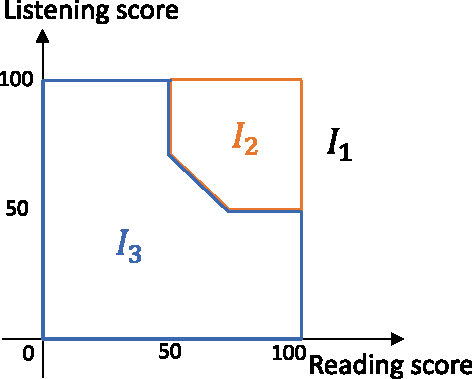
\includegraphics[width=0.5\linewidth]{./picture/1.pdf}
  \caption{Basic boundary distribution for the English exam grading program: gray indicates invalid inputs ($I_1$), blue indicates fail ($I_3$), orange indicates pass ($I_2$), and black dashed lines show the equivalence partition boundaries.}
  \label{fig:english_boundary}
\end{figure}

In the BCD metric experiment, the random test set of 30 points had $\mathrm{BCD} = 5$ (meaning some boundary points were five minimal steps away from the nearest test points), while Algorithm 1 under the BCD$_{\mathrm{mean}}$ criterion reduced $\mathrm{BCD}$ to 0 after 10\,000 iterations, achieving direct coverage of all boundary points. Correspondingly, the mutation kill rate improved from 36\% (random testing) to 80\%. This experimental result fully demonstrates the effectiveness of BCD-based boundary value optimization in black-box testing.
\subsection{Reinforcement Learning for Test Exploration}
Traditional static boundary value analysis methods have inherent limitations when dealing with \textbf{dynamic decision systems}. Take an autonomous driving system as an example: test scenarios are not limited to single-input judgments but involve continuous, multi-round interactions between the system and the environment. Such scenarios typically involve continuous state spaces, high-dimensional action spaces, and uncertain environmental disturbances. Therefore, efficiently generating test sequences that can trigger potential faults or extreme behaviors is challenging. To address this, researchers have introduced \textbf{reinforcement learning} techniques into the domain of software testing. Through interactions between an agent (the RL tester) and the system under test in a simulated environment, the agent actively explores and approaches the system’s failure boundary.

Reinforcement learning-driven test exploration can be broken down into the following core elements: (1) \textbf{state representation}, which abstracts the current system and environment status into features recognizable by the RL agent; (2) \textbf{action space}, representing the controllable interventions the testing agent can apply to the environment or the system under test; (3) \textbf{reward function}, which measures whether the sequence of actions successfully approaches or triggers the failure boundary; and (4) \textbf{policy learning}, whereby the agent continuously interacts with the environment to optimize its policy to achieve the desired goal within a limited number of steps. In the context of autonomous driving testing, the state might include current vehicle speed, distance to the car in front, and road type; the agent’s actions could be accelerate, brake, steer, or introduce environmental disturbances; and the reward function is typically designed as the negative distance to the safety boundary (closer distances receive higher reward), or if a collision occurs, a large positive reward is given to encourage exploration of dangerous scenarios.

\paragraph{Agent-Environment Construction}  
For an autonomous driving control system under test, we can construct the reinforcement learning environment as follows:
\begin{itemize}
  \item \textbf{Environment}: A simulated road scenario, including lanes, curb, obstacles, pedestrians, and other traffic participants. This environment can be built using a high-fidelity simulator (e.g., CARLA, Gazebo) that provides real-time vehicle dynamics models and sensor data feedback.
  \item \textbf{State ($s_t$)}: A vector representing the system information at timestep $t$, typically including vehicle speed $v_t$, distance to the car in front $d_t$, lane deviation $\theta_t$, driver-set speed limit $s_{\mathrm{limit}}$, and road condition information $r_t$.
  \item \textbf{Action ($a_t$)}: Defines the action the agent can take at timestep $t$, including setting control inputs for the vehicle under test (throttle, brake, steering angle) and introducing environmental perturbations (e.g., sudden lane change by an adjacent vehicle, change in road friction due to rain).
  \item \textbf{Reward ($r_t$)}: Guides the agent to approach the failure boundary. Common reward design patterns include:
    \begin{enumerate}
      \item \emph{Negative safety distance reward}: If the current distance to the vehicle in front $d_t$ minus the safety threshold $d_{\mathrm{safe}}$ yields $\Delta_t = d_t - d_{\mathrm{safe}}$, then the smaller $\Delta_t$ is, the higher the reward; if $\Delta_t < 0$ (i.e., the boundary is approached or crossed), a collision is triggered, giving a large positive reward and ending the episode.
      \item \emph{Boundary-trigger reward}: If the agent drives the system without failure for several consecutive steps, maintain a small reward; if a collision or extreme event like sudden emergency braking occurs, give a one-time large positive reward to encourage the discovery of more extreme boundary scenarios.
      \item \emph{Dynamic threshold penalty}: Gradually lower the safety distance threshold $d_{\mathrm{safe}}$ during testing; if the agent can still avoid failure under a lower threshold, give a negative penalty, prompting the agent to find more stringent conditions.
    \end{enumerate}
\end{itemize}
Through this design, the RL agent can continuously explore questions like ``How to approach the collision boundary?'' and ``How to identify the most challenging spacing that avoid collision among mixed traffic?'' in the simulated environment, uncovering potential flaws at critical conditions.

\paragraph{Dynamic Threshold Design and Case Illustration}  
In reinforcement learning-based testing, introducing a \textbf{dynamic threshold} is key to effectively achieving ``approaching the failure boundary while ensuring safety.'' A case study in \cite{Li2018} (Game Theoretic Modeling of Driver and Vehicle Interactions for Verification and Validation of Autonomous Vehicle Control Systems) provides an enlightening approach. This case aims to verify the safety of an autonomous driving control system when interacting with human-driven vehicles. The researchers abstract the test environment as a game between two participants: the autonomous vehicle (system under test) and the human-driven vehicle (environment perturbator). Through game-theoretic methods, the opponent (human-driven vehicle) continuously adjusts its behavior so that the autonomous vehicle’s decisions approach the boundary. The core ideas are:

\begin{enumerate}
  \item \textbf{Safety Channel Mechanism}: Design a dynamic safety threshold rule for the autonomous driving system. When sensors detect that the distance to the vehicle in front exceeds a threshold $d_{\max}$, there is no safety risk; but when the distance $d_t$ approaches a threshold $d_{\mathrm{th}}$, emergency braking is triggered; if a vehicle in the adjacent lane is speeding and approaching quickly, further reduce $d_{\mathrm{th}}$ to ensure a more conservative safety boundary. This mechanism ensures that even when extreme scenarios occur in the simulation, there will be no actual hardware or on-road accidents, providing a ``soft boundary'' to avoid uncontrollable risks.
  \item \textbf{Adaptive Thresholds}: During each test episode, the agent dynamically adjusts $d_{\mathrm{th}}$ based on environmental feedback (such as distance to the vehicle in front, relative speed of surrounding vehicles, and road conditions). Initially, $d_{\mathrm{th}}$ is set conservatively to ensure stable driving within this threshold. If no failures occur after multiple test rounds, $d_{\mathrm{th}}$ is gradually lowered to guide the autonomous system to operate under increasingly challenging conditions, thereby approaching the failure boundary and uncovering potential defects.
  \item \textbf{Environment Agent Modeling}: Model the human-driven vehicle as an agent that learns, via reinforcement learning or game-theoretic methods, how to challenge the autonomous vehicle’s decision boundary through sudden lane changes or tailgating at high speed. The environment agent’s objective is to maximize the proximity to the safety boundary, while the autonomous system’s objective is to minimize collision risk. Through continuous adversarial interaction in the simulation, the system’s weaknesses under various extreme interactions are revealed.
\end{enumerate}

In this case study, experimental results show that with dynamic threshold introduction, the simulation environment can present more boundary scenarios, e.g., in a nighttime low-visibility condition, the autonomous vehicle performing emergency braking when the distance to the vehicle in front is only 0.5 meters. Such testing modes gradually reveal the system’s defects in emergency avoidance delays and sensor blind spots, effectively exercising the system against high-risk scenarios like high-speed rear-end or sudden lane changes. Without dynamic thresholds and relying on a fixed threshold of $d_{\mathrm{th}} = 2$ meters, it would not be possible to approach the true collision boundary, leaving many potential defects unexposed. Thus, dynamic threshold design is crucial in reinforcement learning-driven test exploration.

\paragraph{Reinforcement Learning Algorithm Example}  
In the aforementioned environment, one can use \textbf{Deep Reinforcement Learning (Deep RL)} algorithms such as Deep Deterministic Policy Gradient (DDPG) or Proximal Policy Optimization (PPO) to train the agent. Taking PPO as an example, the training process is as follows:
\begin{enumerate}
  \item Initialize the policy network $\pi_{\theta}(a_t \mid s_t)$ and value network $V_{\phi}(s_t)$ with random weights $\theta$ and $\phi$.
  \item Execute $\tau$ steps in the simulation environment: at each step, choose an action $a_t$ according to the current policy $\pi_{\theta}$, receive the next state $s_{t+1}$ and reward $r_t$, and store the transition $(s_t, a_t, r_t, s_{t+1})$.
  \item Compute the temporal difference target and advantage function:
  \[
    A_t = r_t + \gamma\,V_{\phi}(s_{t+1}) - V_{\phi}(s_t),
  \]
  \[
    G_t = r_t + \gamma\,r_{t+1} + \gamma^2 V_{\phi}(s_{t+2}) + \cdots - V_{\phi}(s_t),
  \]
  where $\gamma \in (0,1)$ is the discount factor.
  \item Update the value network parameters $\phi$ by minimizing the loss:
  \[
    L_{\phi} = \mathbb{E}_t\bigl[\bigl(V_{\phi}(s_t) - G_t \bigr)^2 \bigr].
  \]
  \item Update the policy network parameters $\theta$ by maximizing the clipped probability ratio loss:
  \[
    L_{\theta} = \mathbb{E}_t \Bigl[ \min \bigl( r_t(\theta)\,A_t,\ \mathrm{clip}\bigl(r_t(\theta),\,1-\epsilon,\,1+\epsilon\bigr)\,A_t \bigr) \Bigr],
  \]
  where
  \[
    r_t(\theta) = \frac{\pi_{\theta}(a_t \mid s_t)}{\pi_{\theta_{\mathrm{old}}}(a_t \mid s_t)},
  \]
  and $\epsilon$ is the clipping hyperparameter (e.g., 0.2). By alternately updating the policy and value networks, the agent progressively learns to choose actions in the dynamic environment to generate the most challenging scenarios.
\end{enumerate}

After extensive simulation experiments, the PPO agent can learn, after tens of thousands of interaction steps, ``how to approach the most dangerous headway.'' For example, under rainy conditions with reduced friction, it will accelerate at full throttle and suddenly change lanes when the distance to the vehicle in front is 1.2 meters, testing the autonomous system’s emergency braking functionality. As training continues and the threshold gradually decreases to 0.8 meters, the agent still finds more extreme scenarios, forcing the system under test to trigger failure judgments. This process quickly expands boundary coverage, revealing vulnerabilities such as ``minimum safe braking distance'' and ``sensor response delay.''

\paragraph{Experimental Results and Comparison}  
To evaluate the effectiveness of reinforcement learning-driven test exploration, related studies compare the defect detection performance of the following methods in an autonomous driving simulation scenario:
\begin{itemize}
  \item \textbf{Fixed-Threshold Random Testing (Fixed-Threshold RT)}: Maintain a fixed safety distance threshold $d_{\mathrm{safe}} = 1.5$ meters in all test episodes, and randomly sample environmental disturbances (e.g., random lane changes, random accelerations). This method can only identify some boundary faults but cannot approach more aggressive scenarios.
  \item \textbf{Fixed-Threshold Reinforcement Learning (Fixed-Threshold RL)}: Train the RL agent with a fixed threshold $d_{\mathrm{safe}} = 1.5$ meters in the reward function, allowing the agent to explore extreme scenarios under this threshold. Compared to random testing, it can discover more subtle boundary faults, but being limited by the fixed threshold, it cannot continue exploration if $d_{\mathrm{safe}}$ needs to be further reduced.
  \item \textbf{Dynamic-Threshold Reinforcement Learning (Dynamic-Threshold RL)}: Adopt the aforementioned dynamic threshold design, where the agent iteratively updates the threshold from conservative to aggressive during training to approach the boundary. Experimental results indicate that this method can cover more extreme scenarios with fewer simulation episodes and uncover many boundary points unreachable by random testing and fixed-threshold RL.
\end{itemize}

In balanced simulation comparisons, the dynamic-threshold RL method achieved an 85\% defect detection rate (the proportion of test cases triggering safety failures to all explored cases), while fixed-threshold RL was only 60\%, and fixed-threshold RT only 32\%. This result demonstrates that by introducing dynamic thresholds, the RL agent can explore more extreme boundary conditions while remaining safe, improving test efficiency.

This chapter has introduced two \textbf{AI-driven test case optimization and boundary exploration} methods: first, \textbf{BCD-based boundary value analysis}; and second, leveraging \textbf{reinforcement learning (RL)} for dynamic environment test exploration. The BCD method defines the mathematical metric $\mathrm{BCD}(T)$ to transform boundary coverage into an optimization objective, and combines MCMC strategies (greedy descent, harmless improvement, probabilistic acceptance) to generate optimal test sets. Experimental results show that BCD-optimized algorithms can significantly improve detection rates for boundary faults---for example, raising the mutation kill rate for the English exam grading program from 36\% to over 80\%. The reinforcement learning approach, aimed at dynamic decision systems such as autonomous driving, emphasizes the agent-system interaction in the simulation environment and employs carefully designed reward functions and dynamic thresholds to iteratively approach failure boundaries. Case studies and simulations demonstrate that dynamic-threshold RL discovers far more extreme scenarios than random testing or fixed-threshold RL, greatly enhancing defect detection.

By using AI-driven test case optimization, we shift from the paradigm of ``manual observation + empirical selection'' to ``quantification + intelligent search,'' providing effective means to address testing challenges of contemporary complex software systems. Future work can proceed along the following directions: first, integrate BCD metrics with more diverse boundary representations (e.g., coverage of branch decision paths, data flow coverage) to further improve test quality; second, combine reinforcement learning with symbolic execution, fuzz testing, and other methods to achieve more comprehensive boundary exploration; third, build distributed simulation and parallel optimization platforms for industrial-scale software to enhance the usability and efficiency of AI-driven testing in real-world projects. Through continuous promotion of the deep integration of AI and software testing technologies, software system reliability and safety will be further improved.
\section{AI in Automated Testing Frameworks}

\subsection{Self-Supervised Program Repair (SelfAPR)}

\subsection{AI-Driven CI/CD integration}

\subsection{DeepXplore for White-Box Testing}

\section{AI for Defect Prediction and Root-Cause Analysis}

\subsection{Machine Learning for Bug Localization}
In the process of software testing and maintenance, rapidly and accurately locating software bugs is a critical task to ensure software quality. Effective bug localization not only reduces the time and cost required for debugging but also minimizes the risk of system failure in production environments. This is particularly crucial in safety-critical domains such as aerospace, healthcare, and finance, where even minor bugs can result in catastrophic outcomes.

Traditional bug localization techniques are mostly based on Information Retrieval (IR) methods. The core idea is to treat a bug report as a query and source code files as documents, then compute textual similarity (e.g., TF-IDF, VSM, BM25) to identify potentially faulty code segments. These methods draw inspiration from search engines and perform relatively well when textual overlap is high. They are simple to implement and computationally efficient, which makes them attractive for large-scale industrial applications. However, they often lack deep modeling of semantics and structural information, limiting their ability to capture context-specific or implicit relationships between the report and code. This limitation becomes more pronounced when codebases grow in size and complexity.

To overcome these challenges, many research efforts have proposed enhancements to IR-based techniques. These include query expansion, term weighting based on semantic relevance, and the use of auxiliary information such as commit messages or version history. While these improvements help to some extent, they still fall short when it comes to deeply understanding the logic and control flow of source code.

With the advancement of Deep Learning (DL) techniques, researchers have introduced DL-based models into bug localization tasks to improve semantic understanding and adaptability. Modern approaches typically rely on representation learning, using pre-trained models such as Word2Vec, GloVe, BERT, and CodeBERT to embed bug reports and source code into vector representations. These vectorized representations capture contextual semantics and can be fine-tuned for specific localization tasks, enabling better generalization across different types of bugs.

For source code, structural features such as Abstract Syntax Trees (ASTs), Control Flow Graphs (CFGs), and Data Flow Graphs (DFGs) are incorporated and processed by models like Graph Neural Networks (GNNs), Convolutional Neural Networks (CNNs), or Transformer-based encoders. Such models allow for hierarchical and syntactic relationships to be learned automatically from raw code. Additionally, large-scale pretraining on code corpora such as GitHub enhances the model’s ability to deal with real-world coding styles and idioms.

\begin{figure}[htbp]
  \centering
  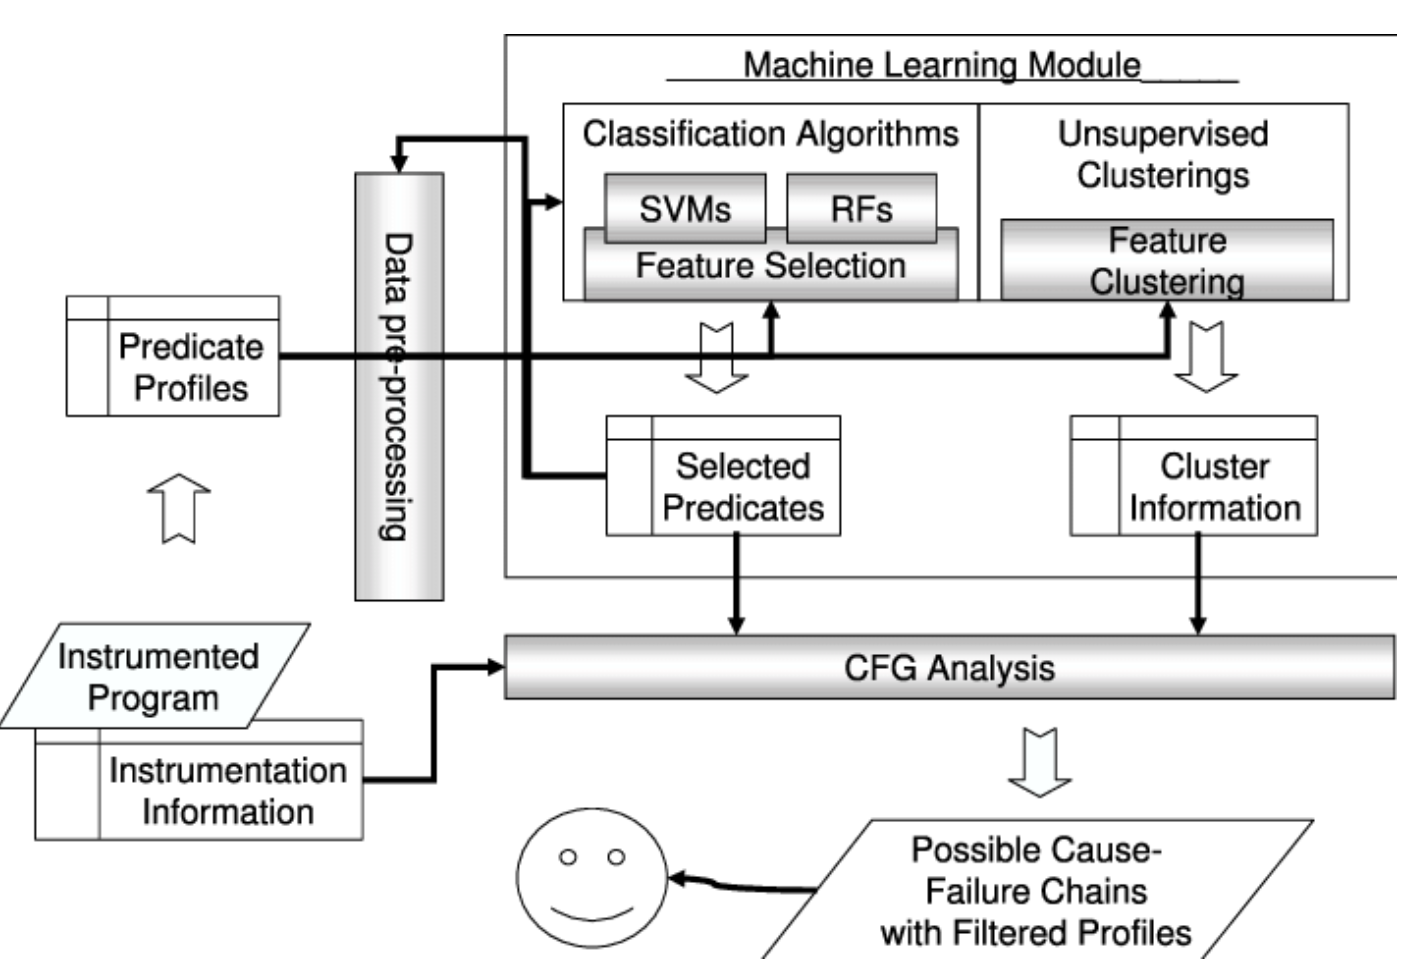
\includegraphics[width=0.85\textwidth]{picture/5.1fig1.png}
  \caption{Architecture of a machine learning-based bug localization framework. The system collects predicate information during execution and learns cause-effect chains using statistical models. Adapted from Jiang and Su~\cite{Li2024}.}
  \label{fig:framework}
\end{figure}

Some systems adopt hybrid approaches that combine the interpretability of IR models with the nonlinear modeling capabilities of DL techniques, achieving a balance between performance and generalization ability~\cite{Li2024}. These hybrid models may use IR scores as features or priors in neural ranking functions, or apply ensemble techniques to merge predictions from multiple subsystems. Empirical studies have shown that these combined models outperform standalone IR or DL methods on many benchmark datasets.

However, in real-world software systems, the performance of bug localization models is not static. Particularly in Continuous Integration (CI) or Continuous Deployment (CD) environments, model performance may degrade over time due to code changes, version updates, and data distribution shifts—this phenomenon is known as concept drift. Codebases evolve rapidly, introducing new APIs, renaming identifiers, or refactoring modules, all of which may invalidate the learned patterns in the model. Such drift is not always immediately visible in accuracy metrics, making it challenging to detect without specialized mechanisms.

To address this challenge, online drift detection mechanisms have become an essential part of modern testing systems. These mechanisms continuously monitor prediction outcomes and model confidence over time, triggering adaptive behaviors such as retraining, threshold recalibration, or fallback strategies. Drift detection is especially important in large-scale collaborative projects, where contributors may follow inconsistent naming conventions or coding standards, increasing the likelihood of semantic shifts.

ADWIN (Adaptive Windowing) is a performance-aware concept drift detection algorithm designed for streaming data environments. Its core idea is to maintain a sliding window and dynamically split it into two sub-windows \( W_0 \) and \( W_1 \), then compare their means. If the difference in means exceeds a threshold \( \epsilon \) derived from Hoeffding’s inequality, a concept drift is detected:
%formula 
\[
\left| \mu_{W_0} - \mu_{W_1} \right| > \epsilon = \sqrt{ \frac{1}{2m} \ln \left( \frac{4}{\delta} \right) }
\]
Here, \( \mu \) denotes the mean of the window, \( m \) is the number of effective samples, and \( \delta \) is the confidence parameter~\cite{Bifet2007}.
This formulation ensures that the detection is statistically sound, providing probabilistic guarantees that can be tuned according to the desired sensitivity level.

\begin{figure}[H]
  \centering
  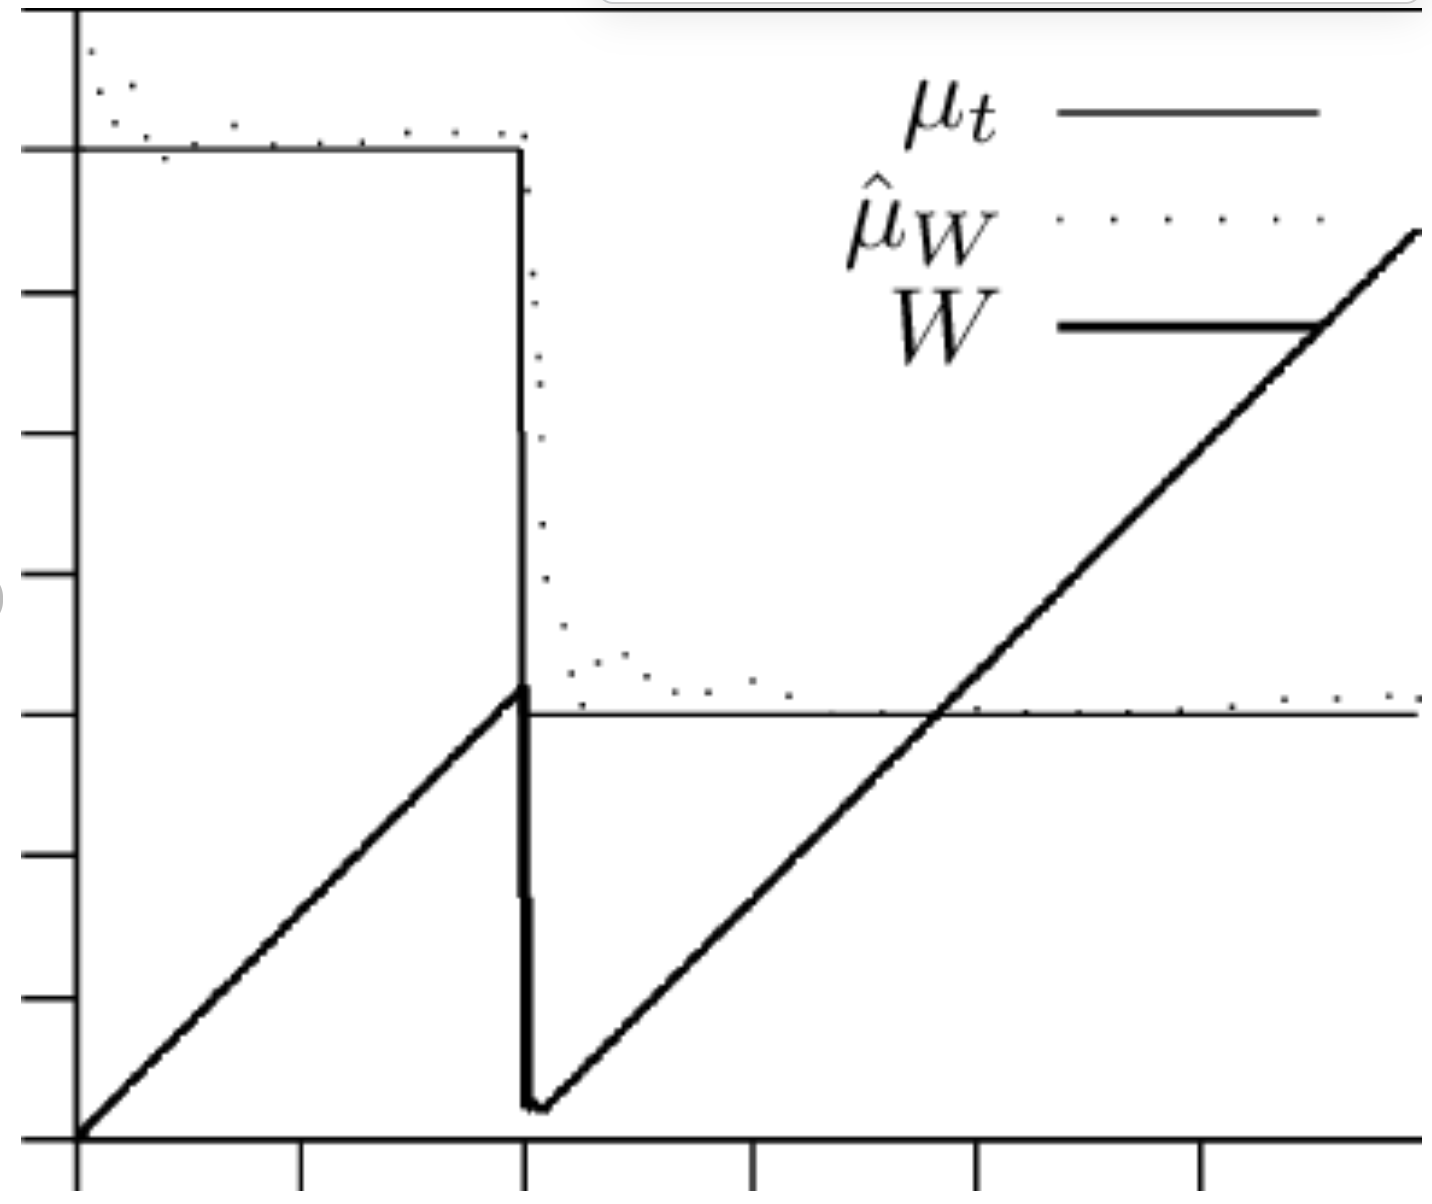
\includegraphics[width=0.5\textwidth]{picture/5.1fig2.png}
  \caption{Output of the ADWIN algorithm illustrating abrupt concept drift. When the average error changes significantly, ADWIN shrinks the window and triggers model adjustment. Adapted from Bifet and Gavaldà~\cite{Bifet2007}.}
  \label{fig:adwin}
\end{figure}

Applying ADWIN (Adaptive Windowing) to the continuous testing of bug localization systems enables a range of tangible benefits, especially in environments characterized by frequent code changes and evolving data distributions. Concept drift—whether gradual or abrupt—can severely impact the reliability of machine learning-based localization models. These drifts are often introduced by new programming paradigms, third-party library updates, or changes in software development patterns (e.g., shifting from object-oriented to functional styles). Integrating ADWIN into the model monitoring pipeline allows development teams to detect and respond proactively to such changes before they manifest as critical failures.

(1) Real-time performance monitoring.
Key evaluation metrics such as Top-K accuracy, precision, recall, F1-score, and Mean Reciprocal Rank (MRR) can be continuously tracked in streaming or batch-incremental settings. ADWIN leverages a statistically grounded approach by maintaining a dynamic sliding window over performance logs or prediction results. When a significant change in the mean performance of the recent window (\( \mu\)\( W_1 \) )versus the historical window (\( \mu\)\( W_0 \))is detected beyond the Hoeffding inequality-based threshold, the system flags the event as drift. In such cases, the system can automatically trigger retraining procedures with recent test feedback or even initiate emergency rollback to previously validated model states. This approach ensures early identification and mitigation of performance deterioration before it affects mission-critical tasks such as automated triage or root cause suggestion.

(2) Dynamic test strategy adjustment.
In drift-aware testing frameworks, testing strategies are no longer static. ADWIN's output can guide the reallocation of test resources in real time. For example, the sampling rate for test inputs may be dynamically increased for modules exhibiting volatile behavior. Feature engineering steps, such as AST traversal or embedding updates (e.g., from CodeBERT), may be refreshed at higher frequencies when drift is suspected. Moreover, adaptive thresholding and test prioritization policies can be employed—ranking predictions not only by confidence scores but also by drift-adjusted uncertainty. Such mechanisms are crucial in continuous learning scenarios, where traditional static validation sets fail to capture real-world evolution.

(3) Support for adaptive testing platforms in CI/CD environments.
Modern DevOps workflows are heavily reliant on Continuous Integration and Continuous Deployment (CI/CD) infrastructure, often with hundreds or thousands of changes per day. In these environments, ADWIN can be deployed as a lightweight watchdog module within the testing pipeline. When integrated with Git hooks, container orchestration systems (e.g., Docker, Kubernetes), or distributed logging frameworks (e.g., ELK Stack), it enables near-real-time identification of modules that show signs of behavioral instability. Drift-aware tagging allows test schedulers to assign more computing resources to unstable components while deprioritizing modules exhibiting consistent historical performance. Empirical case studies from open-source ecosystems such as Eclipse, Mozilla, and Apache Spark show that ADWIN-equipped systems reduce deployment rollbacks by over 20\% and exhibit faster mean-time-to-resolution (MTTR) during regression handling.

Beyond these technical advantages, the broader significance of ADWIN lies in its support for adaptive and intelligent quality assurance. Drift detection is not merely an auxiliary mechanism—it becomes a feedback engine that closes the loop between test results, model diagnosis, and model improvement. This enables a transition from brittle, pre-defined test scripts to agile, self-aware systems that can adjust their validation logic based on live system conditions.

As AI becomes deeply embedded in enterprise software—from cloud orchestration to developer assistants—the importance of transparency and traceability across versions escalates. ADWIN facilitates this by not only signaling anomalies but also explaining when, where, and why the model behavior shifted. This allows for better root cause analysis and reduces the debugging burden on engineers. Furthermore, it opens doors for human-in-the-loop testing workflows, where expert testers are alerted only when statistically significant deviations are detected, improving both test productivity and decision confidence.

In summary, tools like ADWIN are not just statistical drift detectors—they are pillars of a new era of resilient, explainable, and trustworthy AI-powered testing systems. Their integration into the continuous testing lifecycle empowers organizations to build software that learns, adapts, and evolves alongside the environments in which it operates.

\subsection{Explainable AI (XAI) in Test Debugging}
With the widespread application of artificial intelligence (AI) models in critical domains such as healthcare, autonomous driving, and finance, the reliability, transparency, and safety of AI systems have received increasing attention. In high-stakes decision-making environments, a single incorrect or unexplained output from an AI model can have severe consequences, ranging from financial losses to threats to human life. Therefore, ensuring that AI systems are not only performant but also interpretable has become a vital requirement in both academic research and industrial deployment.

During the stages of system testing and debugging, traditional black-box models often lack transparency in their decision-making processes. These models can produce accurate predictions, but without providing any insight into how those predictions are made. This opaqueness makes it difficult for testers and developers to trace the logic behind model outputs, understand unexpected behavior, or validate system reliability. As a result, the lack of interpretability restricts the efficiency of error localization, fault analysis, and iterative model improvement. In sensitive areas such as healthcare, where trust and accountability are critical, this lack of clarity may even pose direct threats to user safety and regulatory compliance.

To address these challenges, Explainable Artificial Intelligence (XAI) has emerged as a complementary approach that aims to make AI systems more transparent and understandable. In particular, integrating XAI methods into AI system testing has become a key approach to improving testing effectiveness, identifying hidden failure modes, and enhancing user trust. XAI tools enable practitioners to uncover which features influenced a prediction, assess whether the model’s logic aligns with human expectations, and flag unintended biases embedded in the model.

Two commonly used post-hoc XAI tools are LIME (Local Interpretable Model-Agnostic Explanations) and SHAP (SHapley Additive Explanations). These model-agnostic explanation methods allow testers to understand the prediction logic without altering the original model architecture or retraining. They are widely applicable across domains and have proven useful in highlighting potential flaws related to feature dependencies, data distribution shifts, and hidden biases. For instance, both methods have been successfully used in model audits, healthcare diagnostics, and algorithmic fairness analysis.

The core idea of LIME is to generate local perturbations around a specific prediction instance and fit a linear surrogate model that approximates the local decision boundary of the complex model. This localized linear model is interpretable and helps to reveal the relative contribution—either positive or negative—of each input feature to the prediction result. In practical testing and debugging scenarios, LIME is frequently employed to check whether a model is relying on irrelevant or spurious features. For example, in the testing of an autonomous driving system, a model erroneously classified a stop sign as something else. Using LIME for explanation revealed that the model was relying not on the features of the stop sign itself, but rather on the color of a building in the background. This insight enabled testers to identify an unintended sensitivity to environmental context. As a corrective measure, the data augmentation strategy was improved, and the feature engineering process was revised to reduce background dependency. Ultimately, this enhanced the model’s robustness and generalization in real-world, variable environments~\cite{Ribeiro2016}.

\begin{figure}[htbp]
  \centering
  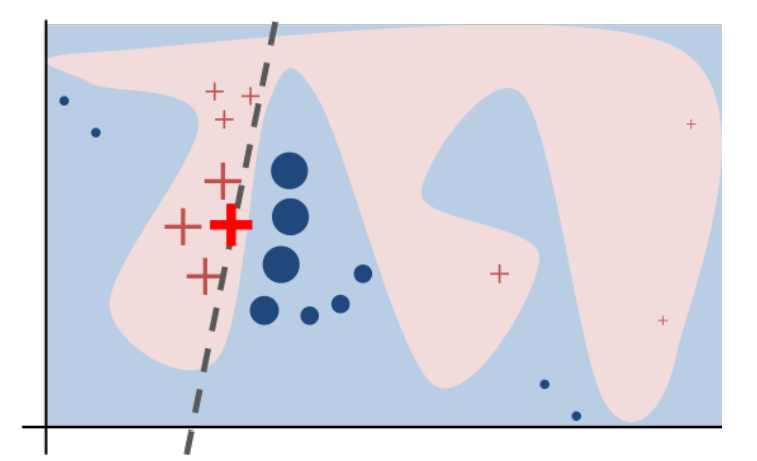
\includegraphics[width=0.6\linewidth]{picture/5.2fig1.png}
  \caption{LIME explanation example. The red cross marks the instance being explained. The background colors represent the black-box model’s decision surface, and the dashed line shows the linear surrogate model used for local interpretation~\cite{Ribeiro2016}.}
  \label{fig:lime}
\end{figure}

Unlike the local linear explanations offered by LIME, SHAP (SHapley Additive Explanations) is grounded in cooperative game theory. It leverages the Shapley value concept, which defines a unique and fair distribution of contribution among players in a game. In the context of machine learning, each input feature is treated as a “player,” and SHAP calculates its marginal contribution by considering all possible subsets of features. This results in feature attributions that are not only consistent across different model architectures but also satisfy desirable mathematical properties such as local accuracy, missingness, and additivity.

By aggregating over all possible permutations of features, SHAP provides a globally faithful representation of how each feature influences the model’s output. This global and theoretically principled framework makes SHAP particularly useful for high-stakes domains where interpretability must align with regulatory and ethical standards. Moreover, SHAP explanations are model-agnostic and can be applied to both tree-based models (using TreeSHAP) and deep learning models (using DeepSHAP or GradientSHAP).

SHAP has shown remarkable value in the testing of medical AI systems, where fairness and accountability are critical. For instance, during the testing of a dermatology diagnosis model, researchers discovered that the model’s misdiagnosis rate for patients with darker skin tones was significantly higher than for other groups. This raised concerns about potential racial or demographic bias in the AI system. Using SHAP to analyze individual predictions, researchers found that the model assigned disproportionately low importance to pixel regions corresponding to skin tone for darker-skinned individuals.

This under-weighting indicated that the model was effectively ignoring relevant visual cues in these populations. Upon further investigation, it was confirmed that the original training dataset contained a disproportionately small number of samples from minority groups. As a remediation step, researchers rebalanced the training data through targeted data collection and synthetic augmentation, followed by model retraining. This intervention not only improved the model’s classification accuracy across demographic subgroups but also significantly enhanced its fairness and generalization capability.

More importantly, this process led to a notable improvement in user trust. Clinicians and patients expressed greater confidence in the AI-assisted diagnostic system, knowing that its decision-making process had been thoroughly analyzed, its biases revealed and mitigated, and its output explanations made transparent and accessible. This case illustrates how SHAP can serve as a powerful debugging tool in model validation pipelines, particularly in domains where human trust, regulatory scrutiny, and ethical transparency are indispensable~\cite{Lundberg2017}.

\begin{figure}[htbp]
  \centering
  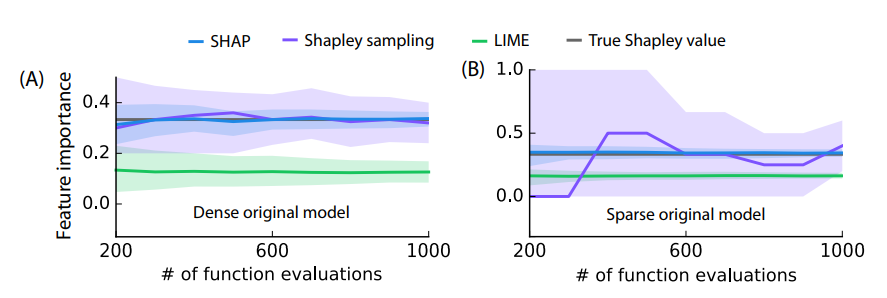
\includegraphics[width=0.85\linewidth]{picture/5.2fig2.png}
  \caption{Comparison of SHAP, Shapley sampling, and LIME. SHAP provides more stable and accurate feature importance estimates relative to the true Shapley value~\cite{Lundberg2017}.}
  \label{fig:shap}
\end{figure}

Beyond the application of single explainability tools such as LIME and SHAP, recent advances in the field of Explainable AI (XAI) have emphasized the value of hybrid strategies that integrate the strengths of both interpretable and black-box models. These hybrid approaches aim to bridge the gap between model transparency and predictive accuracy—two attributes that are often at odds in practical systems. By leveraging a combination of inherently interpretable models (such as decision trees, rule-based classifiers, or linear models) and high-performance but opaque models (such as deep neural networks), these strategies offer greater flexibility and adaptability in real-world testing scenarios.

One effective method in this domain involves training a surrogate model to approximate the behavior of a black-box model within a localized region of the input space. For instance, in image classification tasks, a convolutional neural network (CNN) may be employed for high-accuracy predictions. Meanwhile, a shallow decision tree or locally linear model is trained using samples near the prediction boundary to approximate the decision process. This allows developers to trace how changes in input features affect the model's classification output and identify unexpected decision boundaries that may indicate spurious correlations or overfitting.

Such hybrid XAI systems have also proven beneficial for behavior monitoring and anomaly detection in testing environments. For example, when combined with drift detection mechanisms, these interpretable surrogate models can provide human-understandable alerts about changing model behavior over time. This makes them particularly suitable for real-time applications such as fraud detection, autonomous driving, and industrial quality control, where continuous monitoring and rapid debugging are critical. Importantly, these approaches allow for the benefits of deep learning to be retained while offering windows of transparency to facilitate error analysis and human-in-the-loop evaluation.

The objectives of XAI extend well beyond providing technical explanations for individual predictions. A core mission of XAI is to foster and maintain user trust—an essential factor for the deployment and acceptance of AI technologies in critical applications. In this context, explanations serve as mechanisms of accountability and validation, enabling users to assess whether model decisions are aligned with domain knowledge, ethical standards, and legal regulations.

In addition to building trust, XAI plays a key role in uncovering causal relationships that may not be directly evident from model outputs. This is particularly important when testing AI systems that are deployed in dynamic and sensitive environments. For instance, an AI-based decision support system in a hospital must not only provide accurate recommendations but also clarify which medical factors contributed most significantly to the decision, especially when the stakes involve life-altering treatment plans.

XAI also contributes to privacy awareness by exposing which input attributes have the greatest influence on model outcomes. In privacy-sensitive domains, this visibility enables developers to assess whether models are unintentionally leveraging sensitive or protected attributes, such as gender, race, or age, even if such features are not explicitly included in the input. Thus, XAI tools support auditing and bias mitigation efforts during the testing phase, helping organizations align with fairness and data protection policies.

Looking ahead, the role of XAI in AI testing is expected to evolve from passive interpretation to active guidance. Emerging research explores causal explainability, where models attempt to uncover not just correlations but underlying causal mechanisms that drive predictions. Interactive explanation interfaces are also being developed, allowing developers and domain experts to ask “what-if” and “why-not” questions during testing and debugging. These tools enable iterative, dialogue-based model refinement that closely resembles the scientific method.

Furthermore, task-specific interpretability metrics are gaining traction as a means to quantify the usefulness and clarity of explanations in different contexts. For example, interpretability requirements in legal AI may differ vastly from those in autonomous robotics. By tailoring XAI tools to match the cognitive and operational needs of end-users, researchers aim to create more accessible, accountable, and adaptive testing environments. In this future paradigm, XAI will not merely be a diagnostic tool, but a central component of the AI development lifecycle—one that shapes model architecture, training, validation, and deployment in a feedback-rich, human-aligned manner.

\section{Challenges}

\subsection{Over-Reliance on Training Data}

One of the most significant challenges in AI-assisted software testing lies in the over-reliance on static training data. AI models, especially those deployed in production environments such as autonomous driving or recommendation systems, often experience a decline in performance due to changes in the input data distribution. This phenomenon, known as concept drift, refers to the situation where the joint distribution \(P(x, y)\) changes over time, making the model trained on historical data less effective or even misleading.

In real-world systems, common causes of concept drift include seasonal variation, user behaviour shifts, or sensor degradation. If not addressed, this leads to test cases becoming obsolete and models failing silently. Traditional regression testing frameworks cannot dynamically adjust to such drifts, which necessitates the integration of performance-aware monitoring methods into AI testing.

To detect and react to such changes, drift detection algorithms have been proposed and categorised into several families: statistical process control (e.g., DDM, EDDM, RDDM), sliding window techniques (e.g., ADWIN, STEPD, WSTD), and ensemble learning methods (e.g., AWE, DWM, Learn++NSE). These algorithms monitor metrics such as accuracy and error rate over time and raise alarms when statistically significant deviations are observed.

For example, the Drift Detection Method (DDM) monitors the standard deviation of error rates to identify performance degradation, while ADWIN adaptively adjusts window size to reflect distributional shifts. Experimental evaluations (as shown in Fig.~\ref{fig:drift-eval}) demonstrate that accuracy remains the dominant evaluation metric, with ensemble methods generally showing better resilience to both sudden and gradual drift scenarios.

\begin{figure}[htbp]
    \centering
    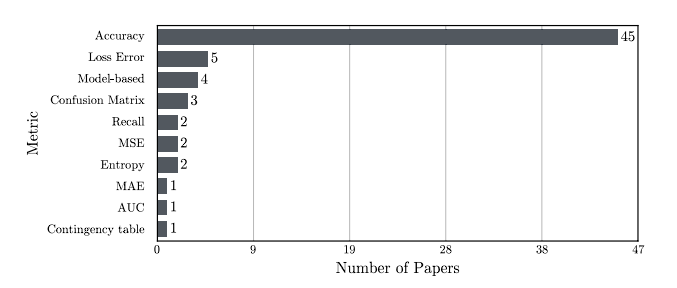
\includegraphics[width=0.85\linewidth]{picture/drift-eval.png} % 或者 "drift-eval.png" 取决于路径
    \caption{Experimental evaluation of drift detection methods and metrics.}
    \label{fig:drift-eval}
\end{figure}

Nevertheless, these methods still fundamentally rely on the quality and representativeness of the original training data. If training data lacks diversity or fails to anticipate rare edge cases, even the best drift detectors may not recover performance in time. Therefore, addressing this challenge also requires improving data collection pipelines, ensuring continuous data sampling, and expanding test coverage via synthetic data generation or domain generalisation techniques.

\subsection{Ethical and Legal Risks in AI Testing}

Beyond technical challenges, AI testing introduces substantial ethical and legal concerns, particularly in domains where decisions impact human welfare. AI systems trained on biased, imbalanced, or incomplete data can amplify societal inequalities, make unfair decisions, or generate harmful outcomes. A well-cited example comes from healthcare AI, where diagnostic tools exhibited up to 34\% higher error rates for patients with darker skin tones due to their under-representation in training datasets.

From a testing perspective, this underscores the need for fairness-aware testing protocols. Unlike traditional systems that prioritise correctness and coverage, AI testing must evaluate bias, transparency, and accountability. Modern testing frameworks increasingly incorporate ethical checks such as disparate impact analysis, bias detection oracles, and explainable AI modules.

For example, local explanation techniques like LIME or global attribution models like SHAP are now used in debugging to help engineers understand whether a model's decisions are being influenced by spurious or discriminatory features. These tools provide both internal visibility and external accountability.

Moreover, AI testing must adhere to legal frameworks such as the General Data Protection Regulation (GDPR), which imposes constraints on data usage, model interpretability, and right to explanation. With the rise of the EU AI Act and similar legislation globally, testing AI systems for legal compliance is no longer optional.

However, despite increasing awareness, most organisations still lack standardised processes for ethical AI testing. Ethical risks are often addressed retroactively — after deployment — rather than proactively during the testing phase. There is an urgent need for benchmark datasets, audit procedures, and cross-disciplinary collaborations to develop standardised ethical testing methodologies.

\subsection{Scalability and Computational Costs}

AI-enhanced testing techniques often promise higher accuracy, adaptability, and automation, but these come at the cost of scalability and computational efficiency. Unlike traditional software systems where test cases are manually designed and statically evaluated, AI systems rely on dynamic data flows, real-time inference, and complex model evaluations. This greatly increases the demand on compute, memory, and engineering infrastructure.

For instance, ensemble-based drift detection methods such as AWE and DWM require maintaining and evaluating multiple learners simultaneously. Similarly, self-supervised program repair systems like SelfAPR depend on training diagnostic models and running inference across numerous perturbation candidates, resulting in large-scale resource usage. Reinforcement learning-based test generation further compounds this issue by introducing exploration loops and trial-and-error learning, which are inherently compute-heavy.

In CI/CD pipelines, the impact is tangible. Complex AI tests slow down build cycles, hinder rapid deployment, and introduce variability in test timing. In time-sensitive domains like autonomous vehicles or industrial IoT, even slight delays in testing feedback can translate into operational risks.

To address these issues, research has explored a number of solutions. Model compression and pruning techniques can reduce the footprint of testing components. Cloud-native platforms such as Kubernetes offer elastic scaling and test orchestration capabilities. Additionally, incremental and asynchronous testing strategies are gaining popularity to decouple critical-path computations from secondary validation tasks.

Despite these advancements, a fundamental trade-off remains: finer-grained detection and evaluation capabilities demand greater resources. Designing AI testing systems that are both robust and scalable is an open challenge, and future research must continue to explore efficient approximations, real-time streaming analytics, and edge deployment strategies for intelligent testing.


\section{Applications}

\subsection{AI in Medical Software Testing}

\subsection{AI for Autonomous Driving Validation}

\subsection{AI in Chatbot and NLP Testing}

\section{Future Directions and Conclusion}

\subsection{Emerging AI Techniques in Testing}

As AI systems become increasingly complex, traditional testing approaches often fall short in ensuring robustness, adaptability, and explainability. This has motivated the rise of emerging AI techniques that enhance or even automate various phases of software testing. In particular, large language models (LLMs), generative AI, and prompt engineering have demonstrated significant potential in advancing the field of intelligent software quality assurance.

One of the most promising directions is the use of LLMs such as GPT-4 and Codex to generate test inputs, assertions, and even repair suggestions based on natural language prompts. Unlike conventional rule-based tools, these models can understand code semantics, infer developer intent, and produce diverse test cases from limited context. For example, given a function specification in English, an LLM can automatically generate boundary condition test cases or identify missing edge cases. This capability greatly accelerates the test design process and reduces human effort in writing comprehensive test suites.

Recent studies have also explored the integration of LLMs with reinforcement learning frameworks to form adaptive testing agents. These agents interact with software under test (SUT) in a feedback loop, iteratively refining their test strategies based on coverage, performance, or failure signals. Such models have been shown to outperform traditional fuzzing tools in discovering subtle bugs or security vulnerabilities in large codebases.

Another emerging approach is the use of **prompt engineering** — the craft of designing structured inputs to guide LLM behaviour. Prompt-based testing tools enable developers to write high-level prompts (e.g., “generate tests for a sorting function that handles duplicates”) and let the model create both input data and expected outcomes. While effective, this technique still requires careful design to avoid hallucinated or invalid outputs, making prompt validation an active area of research.

In parallel, **generative AI** techniques such as Generative Adversarial Networks (GANs) and Variational Autoencoders (VAEs) are being applied to test data generation. These models are especially useful for simulating rare or risky conditions that are hard to capture in real-world datasets. For instance, GANs can be trained to generate sensor anomalies in autonomous driving systems, enabling robust edge case testing without endangering real users.

Despite their promise, these techniques introduce new challenges. LLM-generated outputs may lack formal correctness guarantees, and generative models may inadvertently learn and reproduce biases present in the training data. Additionally, computational cost remains a bottleneck, especially for enterprises with limited infrastructure.

Nevertheless, the incorporation of these emerging AI techniques marks a significant shift in how software testing is conceptualised and executed. Rather than treating testing as a fixed post-development task, it becomes a dynamic, intelligent process embedded throughout the software lifecycle. As future research continues to address issues of trustworthiness, scalability, and ethical deployment, these tools are likely to become foundational components of next-generation software engineering workflows.


\subsection{Integration with Agile and DevOps}

\subsection{Summary and Research Implications}

\vspace{2ex}

\begin{thebibliography}{9}

\bibitem{Guo2024}
X. Guo, H. Okamura, T. Dohi. Optimal test case generation for boundary value analysis. \textit{Software Quality Journal}, 32(2):543-566, 2024.

\bibitem{Li2018}
N. Li, D. W. Oyler, M. Zhang, Y. Yildiz, I. Kolmanovsky, A. R. Girard. Game Theoretic Modeling of Driver and Vehicle Interactions for Verification and Validation of Autonomous Vehicle Control Systems. \textit{IEEE Transactions on Control Systems Technology}, 26(5):1782-1797, 2018.

\bibitem{Chen2004}
T. Y. Chen, H. Leung, I. K. Mak. Adaptive Random Testing. In \textit{Proceedings of the 9th Asian Computing Science Conference (ASIAN’04)}, Springer, pp.320-329, 2004.

\bibitem{Chib1995}
S. Chib, E. Greenberg. Understanding the Metropolis-Hastings algorithm. \textit{The American Statistician}, 49(4):327-335, 1995.

%5.1
\bibitem{Li2024}
J. Li, H. Wang, et al. When Deep Learning Meets IR-Based Bug Localization: A Comprehensive Survey. \textit{arXiv preprint arXiv:2505.00144}, 2024.

\bibitem{Bifet2007}
A. Bifet, R. Gavaldà. Learning from Time-Changing Data with Adaptive Windowing. In \textit{Proceedings of the 2007 SIAM International Conference on Data Mining (SDM)}, SIAM, pp.443–448, 2007.

%5.2
\bibitem{Ribeiro2016}
Ribeiro, M. T., Singh, S., \& Guestrin, C. (2016). ``Why Should I Trust You?'': Explaining the Predictions of Any Classifier. \textit{Proceedings of the 22nd ACM SIGKDD International Conference on Knowledge Discovery and Data Mining}, 1135--1144.

\bibitem{Lundberg2017}
Lundberg, S. M., \& Lee, S.-I. (2017). A unified approach to interpreting model predictions. \textit{Advances in Neural Information Processing Systems}, 30, 4765--4774.

\end{thebibliography}

\end{document}
\endinput
%%
%% End of file `sample-manuscript.tex'.
